\chapter{序論}
\label{chapter1}
宇宙マイクロ波背景放射(Cosmic Microwave Background; CMB)は我々が観測できる宇宙最古の光であり、宇宙初期を知る重要な手がかりとなっている。CMBが持つ温度異方性の観測を基に現代宇宙論の基礎が作られた。しかし、現在の宇宙論には課題があり、地平線問題を始めとする未解決問題が残されている。これらの問題を解決する有力な理論としてインフレーション理論が提唱されている。CMBの偏光にインフレーションの痕跡が残ると考えられており、様々なCMB観測実験が始動している。また、CMBの偏光観測はニュートリノ質量和に対する制限を与えられ、素粒子物理学にも大きな影響を持つ。この章では、CMBとそれを取り巻く宇宙論の関係について述べる。

\section{CMBの温度異方性と現代宇宙論}
%ビッグバン理論は宇宙初期が高温高密度であり、膨張しながら星や銀河を作り、今に至るという宇宙のシナリオを予言した。ビッグバンの証拠には宇宙膨張を示すハッブルの法則やビッグバン元素合成(Big Bang Nucleosynthesis; BBN\cite{BBN})と呼ばれる初期宇宙の軽元素の生成過程が挙げられる。そしてもう1つの証拠はCMBの周波数スペクトルがほぼ\SI{2.725}{K}の黒体放射のスペクトルと一致するという観測事実\cite{2725}である。このことで宇宙初期は熱平衡状態だったことが証明された。

%宇宙初期は高温高密度であり、バリオン物質がイオン化しており、光子は電子と頻繁に散乱される不透明な状況であった。宇宙が膨張して冷えていくにつれてイオンの中性化が進み、電子の個数密度も減少していく。宇宙の温度がおよそ\SI{2970}{K}、宇宙年齢にしておよそ\SI{37}{万年}で光子と電子の散乱率がハッブルパラメータ(宇宙の膨張率)よりも小さくなり、光は散乱されずに真っすぐ進むようになる。この時期を``宇宙の晴れ上がり''または``最終散乱時刻''と呼ぶ\footnote{宇宙の晴れ上がりは光子と電子の散乱率がハッブルパラメータより小さくなる時期、最終散乱時刻はCMB光子が電子と最後に散乱する時刻として定義されるため厳密には異なる時刻を表すが、ほぼ同時刻とみなしてもよい}。我々観測者は最終散乱時刻に対応する``最終散乱面''に囲まれており、そこから散乱されることなく届くCMB光子を観測することができる。

\subsection{CMBの温度異方性}
ビッグバン理論は宇宙初期が高温高密度であり、膨張しながら星や銀河を作り、今に至るという宇宙のシナリオを予言した。ビッグバンの証拠には宇宙膨張を示すハッブルの法則やビッグバン元素合成(Big Bang Nucleosynthesis; BBN\cite{BBN})と呼ばれる初期宇宙の軽元素の生成過程が挙げられる。そしてもう1つの証拠はCMBの周波数スペクトルがほぼ\SI{2.725}{K}の黒体放射のスペクトルと一致するという観測事実\cite{2725}である。このことで宇宙初期は熱平衡状態だったことが証明された。

宇宙初期は高温高密度であり、原子が電子と原子核に電離していた。そのため光子は電子と頻繁に散乱される不透明な状況であった。宇宙が膨張して冷えていくにつれてイオンの中性化が進み、電子の個数密度も減少していく。宇宙の温度がおよそ\SI{2970}{K}、宇宙年齢にしておよそ\SI{37}{万年}で光子と電子の散乱率がハッブルパラメータ(宇宙の膨張率)よりも小さくなり、光は散乱されずに真っすぐ進むようになる。この時期を``宇宙の晴れ上がり''または``最終散乱時刻''と呼ぶ\footnote{宇宙の晴れ上がりは光子と電子の散乱率がハッブルパラメータより小さくなる時期、最終散乱時刻はCMB光子が電子と最後に散乱する時刻として定義されるため厳密には異なる時刻を表すが、ほぼ同時刻とみなしてもよい。}。我々観測者は最終散乱時刻に対応する``最終散乱面''に囲まれており、そこから散乱されることなく届くCMB光子を観測することができる。

CMBがほぼ\SI{2.725}{K}の黒体放射のスペクトルを持つと同時にわずかな温度異方性を持つことも発見された。ある空の1点でのCMB温度を$T(\theta,\phi)$とする。全方向で平均した温度は
\begin{equation}
  \langle T \rangle = \frac{1}{4\pi}\int T(\theta,\phi)\sin\theta d\theta d\phi = \SI{2.725}{\mathrm{K}}
\end{equation}
である。この空の1点$(\theta,\phi)$における温度揺らぎを
\begin{equation}
  \frac{\Delta T}{T}(\theta,\phi) \equiv \frac{T(\theta,\phi) - \langle T \rangle}{\langle T \rangle}
\end{equation}
と定義する。Planck衛星によって観測された温度揺らぎ\cite{Planck_T}は$\sim \SI{100}{\mu\mathrm{K}}$であり、わずかな温度異方性を示している(図\ref{Planck_T})。

\begin{figure}[htbp]
  \centering
  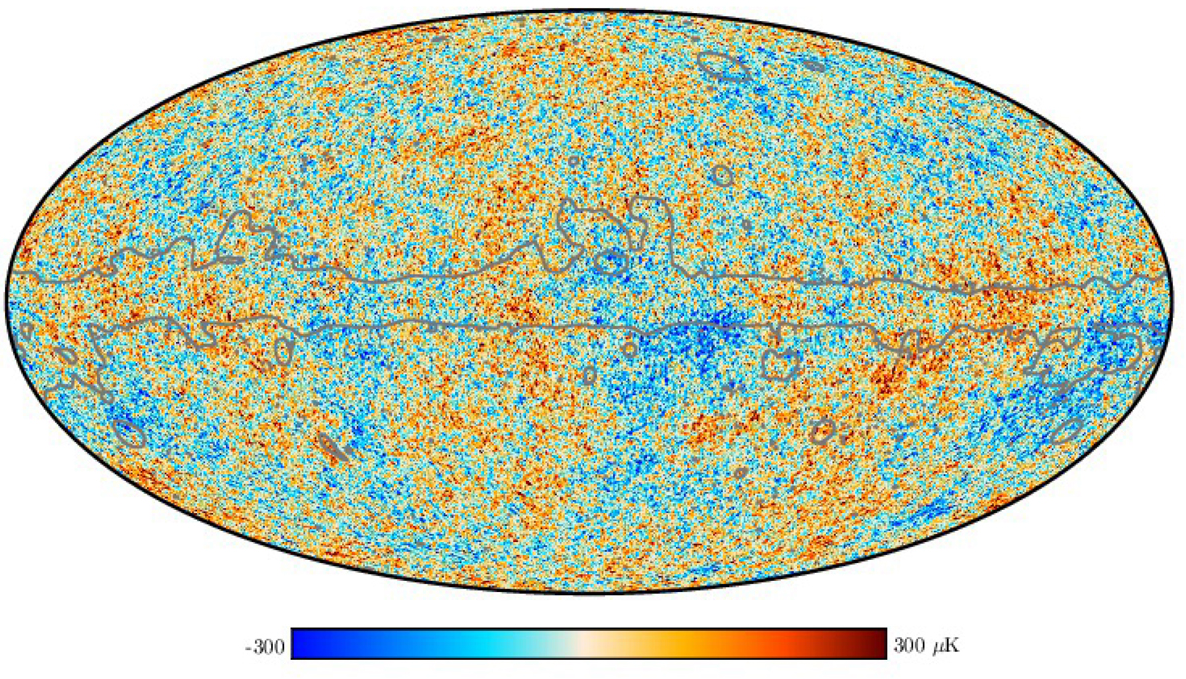
\includegraphics[width=0.85\columnwidth]{2_cosmology/figs/planck_T_map_single.png}
  \caption{Planck衛星によって観測されたCMBの温度異方性のマップ。}
  \label{Planck_T}
\end{figure}
CMB実験ではCMBの観測データと望遠鏡の角度データを用いて図\ref{Planck_T}で示すようなCMBの異方性を表す``マップ(強度分布図)''を作成する。このマップを球面調和関数$Y^{m}_{\ell}(\theta,\phi)$で展開してパワースペクトル($C_{\ell}$)作成することで、宇宙論パラメータを求めることができる。空(天球面上)の$(\theta,\phi)$(図\ref{kyuuzahyou})に対して単位ベクトル$\hat{n}$を
\begin{equation}
  \hat{n} \equiv (\sin\theta\cos\phi,\sin\theta\sin\phi,\cos\theta)
\end{equation}
と定義する。
\begin{figure}[htbp]
  \centering
  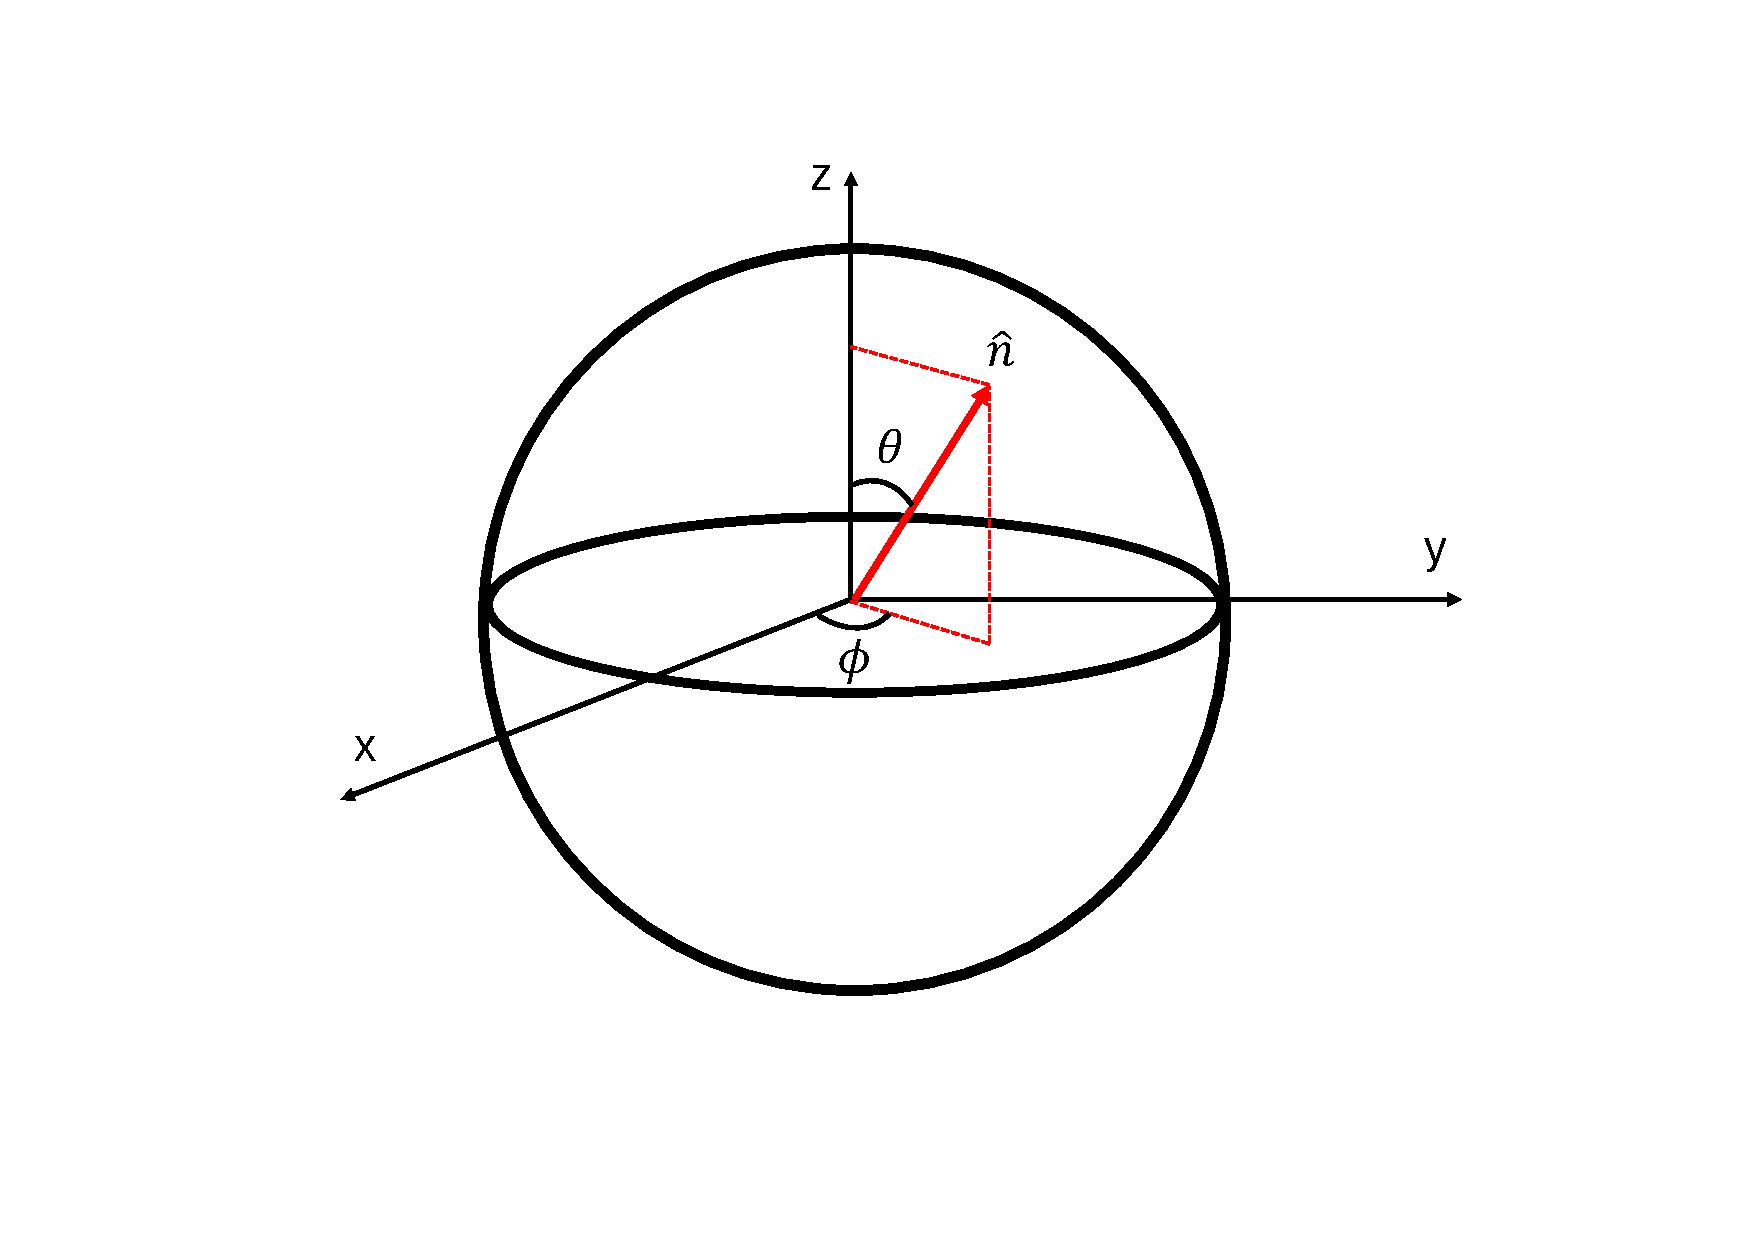
\includegraphics[width=0.5\columnwidth]{2_cosmology/figs/kyuuzahyou.pdf}
  \caption{天球面の座標。}
  \label{kyuuzahyou}
\end{figure}
この時、CMBの温度異方性$\Delta T(\hat{n})\equiv T(\hat{n}) - \langle T \rangle$を球面調和関数で
\begin{equation}
  \Delta T(\hat{n}) = \sum_{\ell=1}^{\infty}\sum_{m=-\ell}^{\ell}a_{\ell m}Y^{m}_{\ell}(\hat{n})
\end{equation}
と展開する。ここで、$a_{\ell m}$は展開係数である。また、$m$は揺らぎの方向を決め、$\ell$は揺らぎのスケールの大きさを表す。$\ell$と角度スケール($\delta\theta$)の関係は
\begin{equation}
  \delta\theta = \SI{180}{^{\circ}}/\ell
\end{equation}
と表せる。しかし、展開係数$a_{\ell m}$は添字$m$による座標依存性があるため、パワースペクトル$C_{\ell}$は展開係数$a_{\ell m}$に対して
\begin{equation}
  C_{\ell}\equiv\frac{1}{2\ell+1}\sum_{m=-\ell}^{\ell}a_{\ell m}{a^{\ast}_{\ell m}}
\end{equation}
と定義することで、座標に依らない物理量として扱うことができる。

\subsection{$\Lambda$-CDMモデル}
CMBのパワースペクトルの測定により、$\Lambda$-CDMモデルと呼ばれる宇宙の進化を記述する標準理論が構築された(図\ref{fit_planck})。$\Lambda$-CDMモデルは、6つのパラメータのみで宇宙を記述するもので、$\Lambda$はダークエネルギーに対応するアインシュタインの宇宙定数を表し、CDMは``Cold Dark Matter''を意味する。
\begin{figure}[htbp]
  \centering
  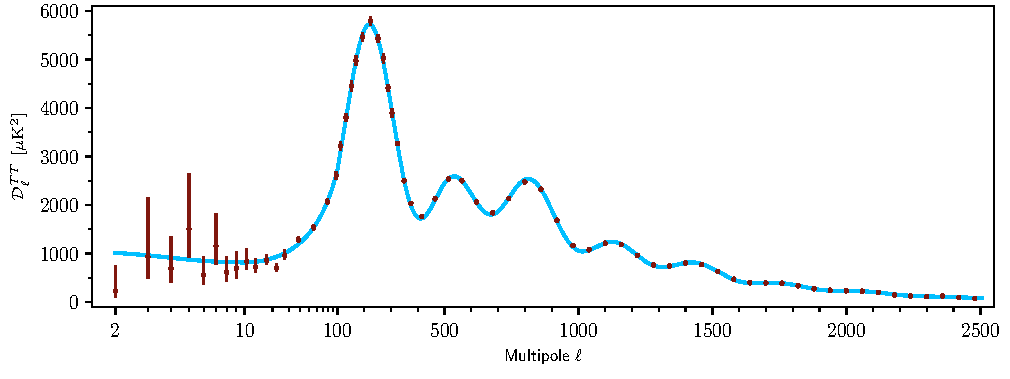
\includegraphics[width=0.85\columnwidth]{2_cosmology/figs/plank_cltt.pdf}
  \caption{Planckの観測から計算されたCMBの温度パワースペクトル\cite{Planck_T}。縦軸の$\mathcal{D}^{TT}_{\ell}$は$\mathcal{D}^{TT}_{\ell} = \frac{\ell(\ell+1)C_{\ell}}{2\pi}$を表す。青の線は$\Lambda$-CDMモデルのベストフィットを表す。}
  \label{fit_planck}
\end{figure}
現在での$\Lambda$-CDMモデルのパラメータを表\ref{6params}にまとめる。
\vspace{2mm}
\begin{table}[htbp]
  \centering
  \caption{Planckの観測から得られた$\Lambda$-CDMモデルの宇宙論パラメータ\cite{Planck_T}。
  これらの値の推定にはCMBの偏光、lensingのパワースペクトル、バリオン音響振動も用いる。}
  \vspace{2mm}
  \begin{tabular}{l|l}\hline
    $\Omega_{b} h^2$ ~(バリオン密度)& 0.02242 $\pm$ 0.00014 \\
    $\Omega_{c} h^2$ ~(CDM密度)& 0.11933 $\pm$ 0.00091 \\
    $100\theta_{MC}$ ~(最終散乱面の見込み角度) & 1.04101 $\pm$ 0.00029 \\
    $\tau$ ~(再電離期における光学的厚み)& 0.0561 $\pm$ 0.0071 \\
    $ln(10^{10}A_s)$ ~(スカラー型の原始揺らぎの振幅) & 3.047 $\pm$ 0.014 \\
    $n_s$ ~(スカラー型の原始揺らぎのべき係数)& 0.9665 $\pm$ 0.0038 \\ \hline
  \end{tabular}
  \label{6params}
\end{table}
現在では我々の知っているバリオン物質はエネルギー密度でたったの$\SI{5}{\%}$で、ダークエネルギーが約$\SI{70}{\%}$、CDMが$\SI{25}{\%}$を占めている。一方で、宇宙初期では異なるエネルギー密度の組成を持っている。

$\Lambda$-CDMモデルにおける一様等方な宇宙では、エネルギー密度$\epsilon(t)$、圧力$P(t)$、スケールファクター\footnote{時刻$t$での宇宙の広がりを表す膨張因子}$a(t)$の関係は、フリードマン方程式\footnote{本論文では$\hbar=c=1$の自然単位系を用いる。}
\begin{equation}
  \left(\frac{\dot{a}}{a}\right)^2 = \frac{8\pi G}{3}\epsilon -\frac{K}{a^2} + \frac{\Lambda}{3} \label{eq:friedmann}
\end{equation}
と、流体方程式
\begin{equation}
  \dot{\epsilon} + 3\frac{\dot{a}}{a}(\epsilon + P) = 0 \label{eq:flow}
\end{equation}
と、状態方程式
\begin{equation}
  P = \omega\epsilon \label{eq:eos}
\end{equation}
で表せる\cite{nyuumonn}。ここで$G$はニュートンの重力定数である。また、$K$は空間曲率を表し、$K=0$で平坦宇宙を表す。$\omega$は宇宙を占める成分ごとに異なるパラメータであり、成分は
\begin{itemize}
  \item 放射(相対論的粒子、$\omega=\frac{1}{3}$)
  \item 物質(非相対論的粒子、$\omega$ = 0)
  \item ダークエネルギー($\omega = -1$)
\end{itemize}
に分けられる。各成分ごとに方程式が成り立つとすると、式\eqref{eq:flow}と式\eqref{eq:eos}から成分$i$のエネルギー密度は
\begin{equation}
  \epsilon_{i}(a) = \epsilon_{i,0}a^{-3(1+\omega_{i})} \label{eq:energy_density}
\end{equation}
となる。ここで、$\epsilon_{i,0}$は現在での値である。$a$は宇宙初期では0に近づくため、$\omega$が大きい成分ほど優勢になる。逆に宇宙の膨張するにつれて$\omega$が小さい成分ほど優勢になる。そのため、現在ではダークエネルギー優勢であるが、宇宙の初期では放射や物質が優勢であった。

放射、物質優勢宇宙でのスケールファクターの時間依存性を見る。成分$\omega$の1成分宇宙でかつ平坦であると仮定すると式\eqref{eq:friedmann}は以下の単純な形になる。
\begin{equation}
  \dot{a}^{2} = \frac{8\pi G\epsilon_{0}}{3}a^{-(1+3\omega)}
\end{equation}
スケールファクターが$a\propto t^{q}$の冪乗に従うと仮定すると
\begin{equation}
  a(t) \propto t^{2/(3+3\omega)}
\end{equation}
で表せる。したがって放射優勢期、物質優勢期では宇宙は減速膨張であったことが分かる(表\ref{rad_vs_mat})。

ダークエネルギー優勢宇宙では式\eqref{eq:energy_density}から、エネルギー密度は一定であり、式\eqref{eq:friedmann}を解くことで
\begin{equation}
  a(t) \propto e^{Ct} ~ (C = \mathrm{Const})
\end{equation}
を得られ、宇宙は加速膨張する。
\begin{table}[htbp]
  \centering
  \caption{エネルギー成分ごとのスケールファクターの時間依存性。}
  \vspace{3mm}
  \begin{tabular}{ccc} \hline
    エネルギー成分 & $a(t)$ & $\ddot{a}(t)$ \\ \hline
    放射 & $t^{1/2}$ & $< 0$ \\
    物質 & $t^{2/3}$ & $< 0$ \\
    ダークエネルギー & $e^{Ct}$ & $> 0$ \\ \hline
  \end{tabular}
  \label{rad_vs_mat}
\end{table}

\subsection{地平線問題}
平坦な空間を動径$r$方向に進む光の経路は$ds^{2} = -dt^{2} + a^{2}(t)dr^{2} = 0$であり、これより光子が到達できる共動距離(宇宙の膨張に依らない距離)は
\begin{equation}
  r = \int_{0}^{r}dr' = \int_{0}^{t}\frac{1}{a(t')}dt'
\end{equation}
となる。これにスケールファクターをかけて物理的距離にすると
\begin{equation}
  d_{\mathrm{hor}}(t)\equiv a(t)r = a(t)\int_{0}^{t}\frac{1}{a(t')}dt' \label{eq:horizon}
\end{equation}
を得る。この$d_{\mathrm{hor}}(t)$を``地平距離''と呼び、ある時刻$t$までに光が到達できる距離、すなわちある時刻$t$で相関を持てる距離を表す。放射優勢期では、表\ref{rad_vs_mat}のスケールファクターを式\eqref{eq:horizon}に代入すると$d_{\mathrm{hor}}(t) = 2t$となる。物質優勢期でも同様にして$d_{\mathrm{hor}}(t) = 3t$を得られる。つまり、減速膨張宇宙では地平距離は$t$に比例して増加する。これは宇宙初期では地平距離が宇宙の膨張よりも速く広がることを意味する。CMBは最終散乱時刻での散乱光であるが、最終散乱時の地平距離は天球上の見込み角で約$\SI{2}{^{\circ}}$しかない。すなわち、$\SI{2}{^{\circ}}$以上離れた領域同士は地平距離より離れており、相関を持てない。一方で、CMBの温度異方性は図\ref{Planck_T}のように$\SI{100}{\mu\mathrm{K}}$の精度で等方的であり、相関を持たないはずの領域まで温度が一致している。既存の理論ではこの観測結果を説明することはできず、``地平線問題''と呼ばれる。この他にも宇宙初期で極端に平坦であったという``平坦性問題''や、モノポール(磁気単極子)が存在しない``モノポール問題''などが未解決な問題となっており、新たな理論による説明が求められる。

\section{CMBの偏光とインフレーション理論}

\subsection{インフレーション理論}
地平線問題をはじめとする現在の宇宙論が抱える問題を解決する有力な理論として``インフレーション理論''が提唱されている。この理論はビッグバンより前の初期に宇宙が加速膨張したとする理論である。加速膨張によって地平距離が大きく引き伸ばされ、最終散乱面全体で相関を持てるようになり、CMB温度異方性の観測結果を説明することができる。表\ref{rad_vs_mat}にあるように、ダークエネルギーのように働く機構があれば加速(指数関数的)膨張を実現できる。インフレーションではインフラトンと呼ばれるスカラー場を導入して加速膨張を説明する。インフラトン$\phi$が一様な空間でポテンシャル$V$を持つとすると、エネルギー密度は
\begin{equation}
  \epsilon_{\phi} = \frac{1}{2}\dot\phi^{2} + V(\phi) \label{eq:energy_phi}
\end{equation}
となり、インフラトン場の圧力は
\begin{equation}
  P_{\phi} = \frac{1}{2}\dot\phi^{2} - V(\phi) \label{eq:pressure_phi}
\end{equation}
で与えられる。インフラトン場が
\begin{equation}
  \dot\phi^{2} \ll V(\phi) \label{eq:condition}
\end{equation}
のようにゆっくり変化する時、インフラトン場はダークエネルギーのように振る舞う。すなわち、インフレーションを起こすための条件は
\begin{itemize}
  \item $\dot\phi$が十分小さい
  \item $\epsilon_{\phi}\sim V(\phi)$が大きく、優勢である
\end{itemize}
である。

初期宇宙でこの条件をどう満たすのかを見る。式\eqref{eq:flow}より、インフラトン場の流体方程式は
\begin{equation}
  \dot\epsilon_{\phi} + 3H(t)(\epsilon_{\phi} + P_{\phi}) = 0  ~~ (H(t) = \dot{a}/a)
\end{equation}
である。これに式\eqref{eq:energy_phi}と式\eqref{eq:pressure_phi}を代入すると
\begin{equation}
  \ddot\phi + 3H(t)\dot\phi + \frac{dV}{d\phi} = 0
\end{equation}
を得る。これは摩擦力を受ける粒子の運動方程式と同じであり、$3H(t)\dot\phi$が摩擦項に対応する。インフラトン場が``終端速度''に達した($\ddot\phi = 0$)時に
\begin{equation}
  \dot\phi = -\frac{1}{3H}\frac{dV}{d\phi}
\end{equation}
となる。これより、式\eqref{eq:condition}の条件は
\begin{equation}
  \Bigl(\frac{dV}{d\phi}\Bigr)^{2} \ll 9H^{2}V
\end{equation}
に置き換えられる。すなわち、インフラトンポテンシャルの勾配が十分小さく、摩擦項が十分大きければインフラトン場は加速膨張を引き起こすことができる。この条件は``スローロール条件''と呼ばれる(図\ref{slow_roll})。
\begin{figure}[htbp]
  \centering
  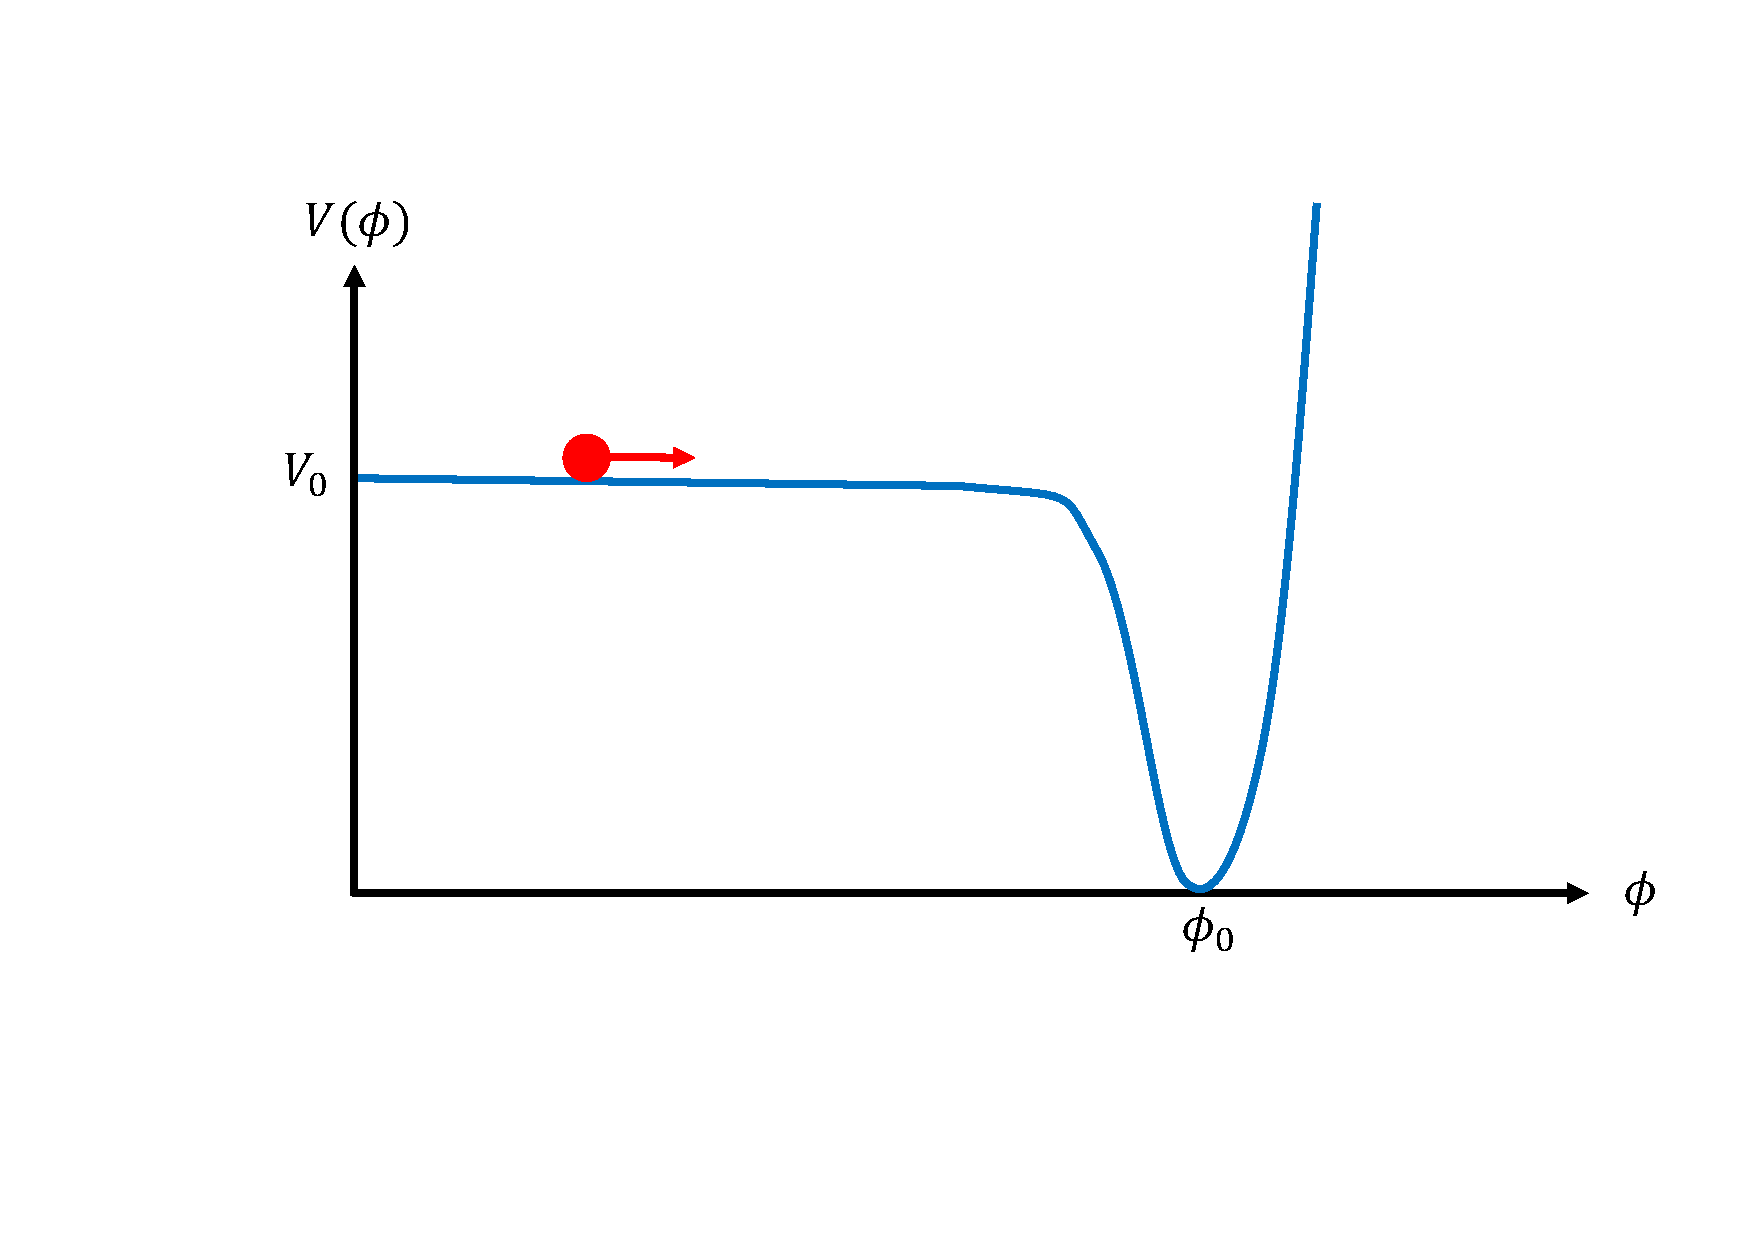
\includegraphics[width=0.8\columnwidth]{2_cosmology/figs/slow_roll.pdf}
  \caption{インフレーションを起こせるポテンシャルの例。ポテンシャルの最小値は$\phi = \phi_{0}$であり、$\phi$は$\phi_{0}$に向けてゆっくりと転がっていく。その間、インフラトン場は一定のエネルギー密度$\epsilon_{\phi}\sim V_{0}$として加速膨張に作用する。}
  \label{slow_roll}
\end{figure}

\subsection{CMBの偏光モード}
インフレーション理論は宇宙の加速膨張を説明するが、その際に原始重力波が生成されると考えられている\cite{primordial}。この原始重力波はCMBに空間非対称な``Bモード''と呼ばれる偏光パターンを残す。つまり、CMBの偏光Bモードを観測することでインフレーション理論の検証が可能になる。

まず、CMBの偏光が生成される原理を説明する。CMBに偏光ができるには
\begin{itemize}
  \item トムソン散乱
  \item 電子から見た四重極の温度異方性
\end{itemize}
の2つが鍵となる\cite{komatsu}。CMBの偏光は図\ref{cmb_tom}で示すように電子とのトムソン散乱によって生まれる。
\begin{figure}[htbp]
  \centering
  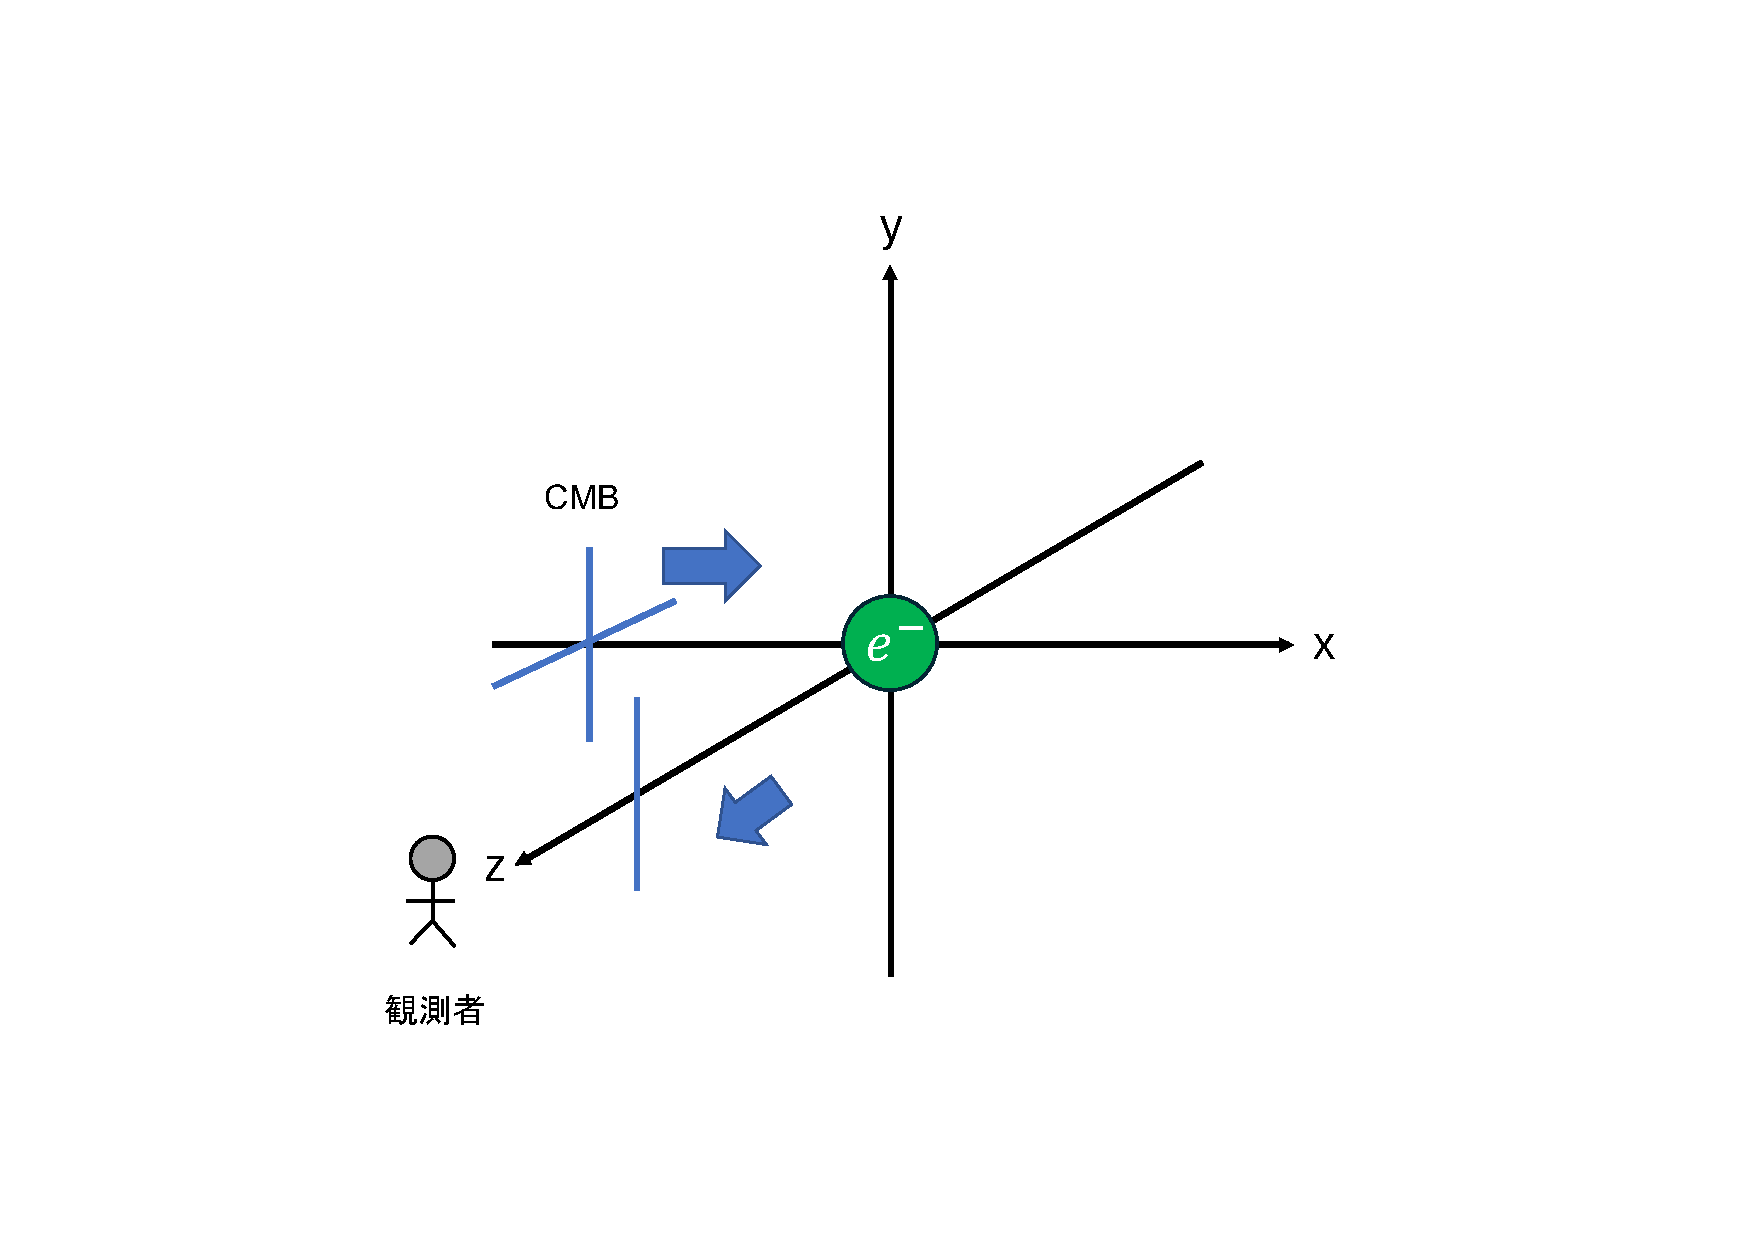
\includegraphics[width=0.8\columnwidth]{2_cosmology/figs/pol_1.pdf}
  \caption{偏光が生じる原理。$x$軸方向に入射する無偏光であった光が$z$軸方向(観測者のいる方向)に散乱されると、$y$軸方向の直線偏光のみが残る。}
  \label{cmb_tom}
\end{figure}
実際にはあらゆる方向から入射する光が電子と散乱されるため、光の温度が等しければ重ね合わせによって無偏光として観測される。しかし、CMBにはわずかな温度異方性があり、電子の静止系において四重極の温度異方性があれば偏光を観測できる(図\ref{four_pol})。
\begin{figure}[htbp]
  \centering
  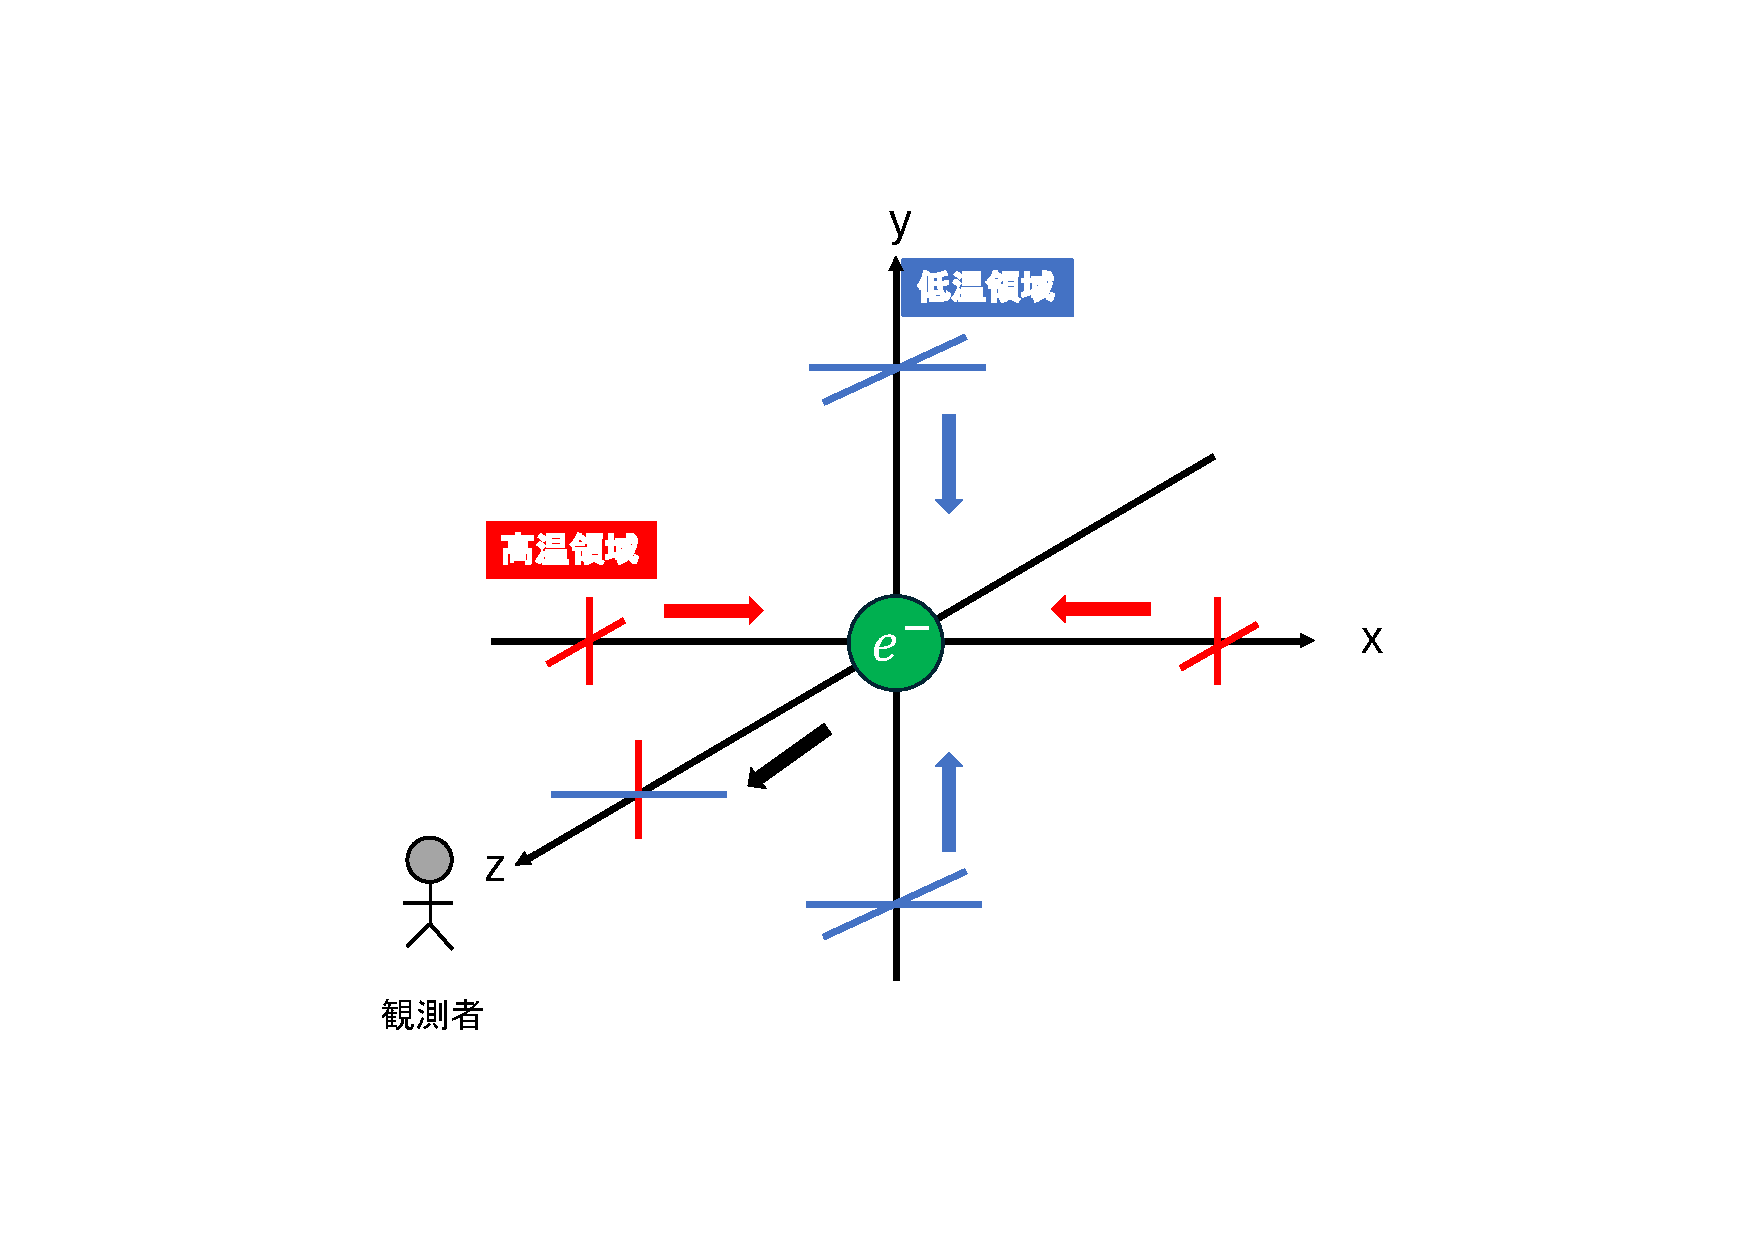
\includegraphics[width=0.8\columnwidth]{2_cosmology/figs/pol_2.pdf}
  \caption{電子の静止系で四重極の温度異方性によって作られる直線偏光。高温領域と低温領域が$\SI{90}{^{\circ}}$ごとに分布する時、直線偏光を観測できる。}
  \label{four_pol}
\end{figure}

CMBの偏光を表す観測量として、デカルト座標軸$(x,y)$と、それに対して$\SI{45}{^{\circ}}$傾けた$(a,b)$軸をとり、各軸での電場成分に対してストークスパラメータ$Q,U$を
\begin{align}
  Q &\propto E_{x}^{2} - E_{y}^{2} \\
  U &\propto E_{a}^{2} - E_{b}^{2}
\end{align}
と定義する。しかし、この量は観測者の系の取り方によって変化するため、$Q,U$を組み合わせて観測者の系に依存しない偏光成分としてEモードとBモードを定義する(図\ref{pol_mode})。ある波数ベクトル$\bm{\ell}$が作る偏光分布を考える時、Eモード偏光は$\bm{\ell}$に平行か垂直であり、空間対称である。一方で、Bモード偏光は$\bm{\ell}$に対して$\SI{45}{^{\circ}}$傾いており、空間非対称である。これによって偏光成分を区別できる。
\begin{figure}[htbp]
  \centering
  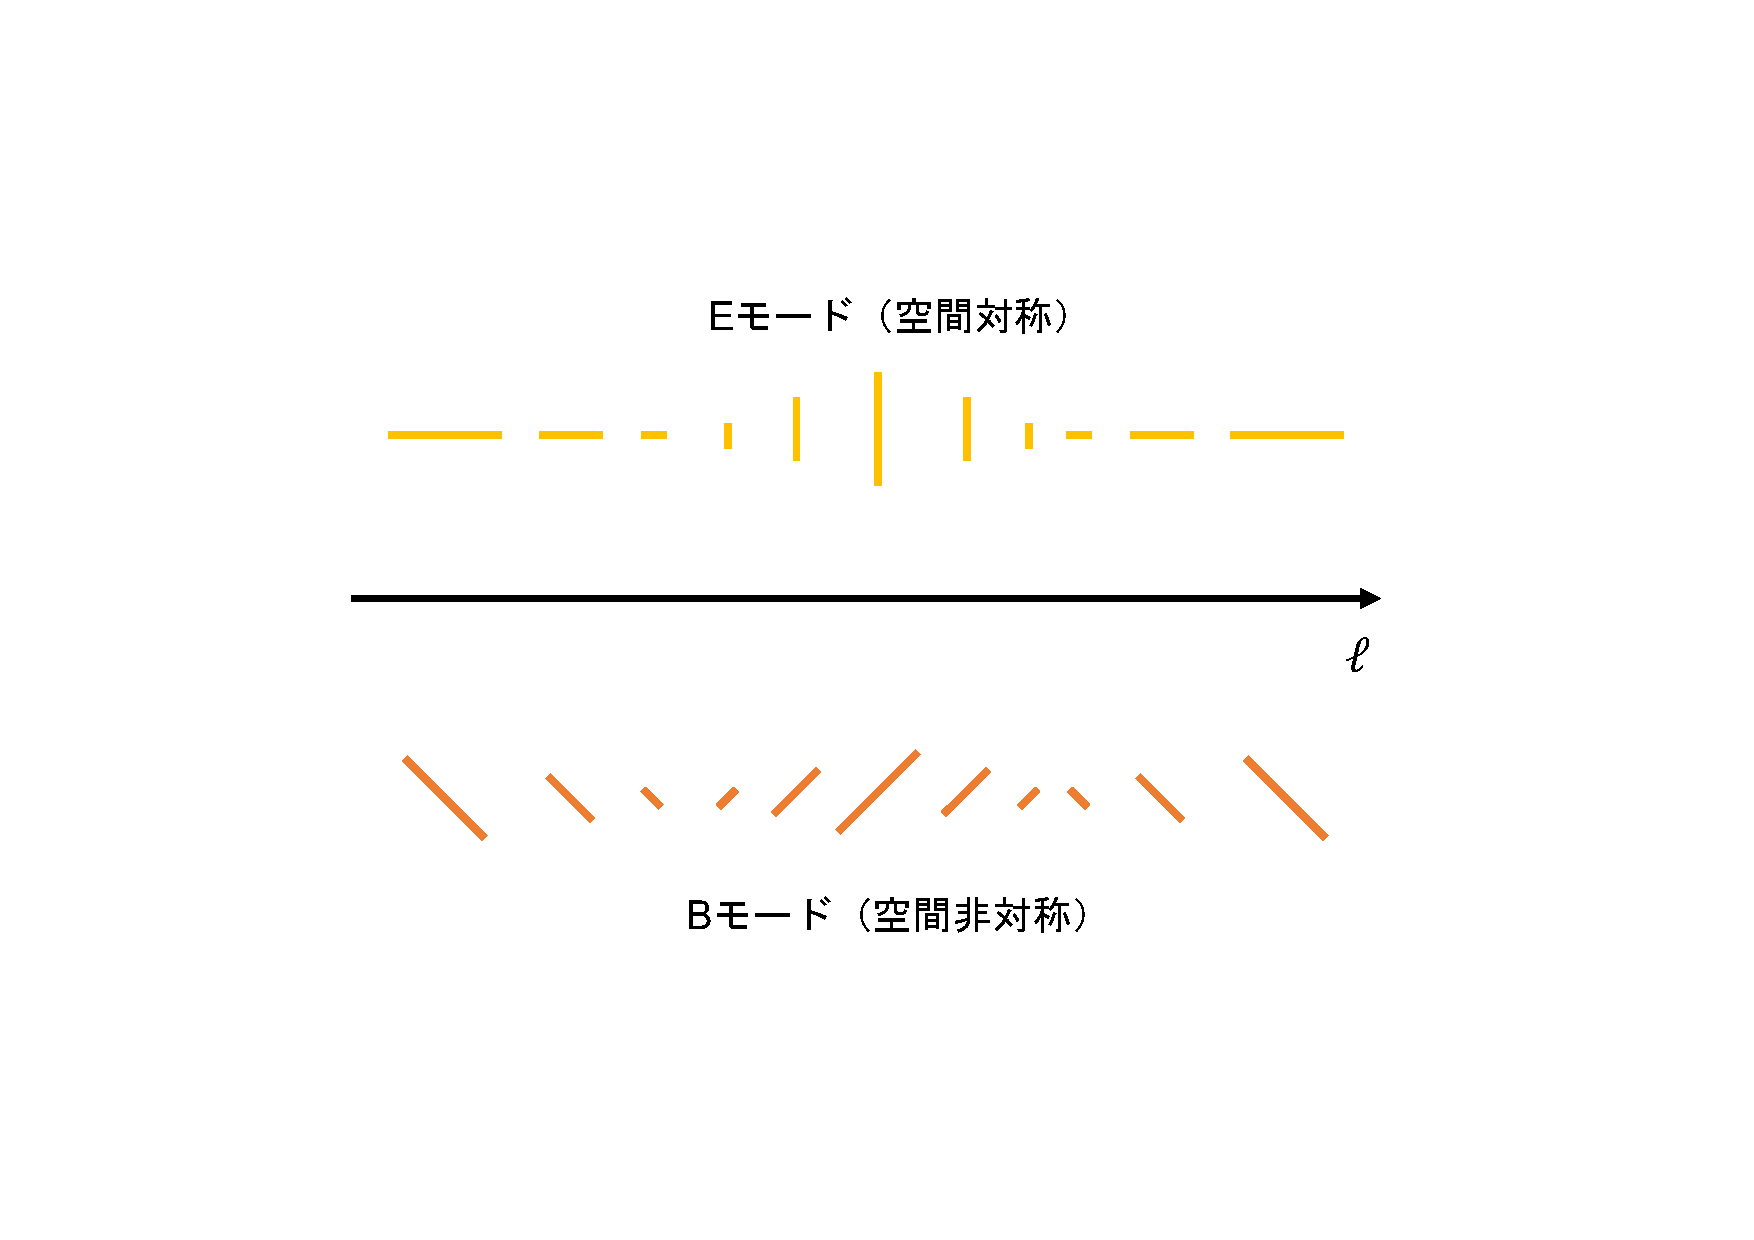
\includegraphics[width=0.8\columnwidth]{2_cosmology/figs/pol_mode.pdf}
  \caption{波数ベクトル$\bm{\ell}$に対する偏光EモードとBモード。線の長さがストークスパラメータの大きさに対応する。}
  \label{pol_mode}
\end{figure}

偏光Bモードは原始重力波と重力レンズ効果の2つの要因から生成される。CMBに異方性をもたらすインフラトンの揺らぎは``スカラー型揺らぎ''と``テンソル型揺らぎ''に分けられ、原始重力波はテンソル型揺らぎに対応する\footnote{一方で、スカラー揺らぎは偏光Eモードのみを生成する}。重力レンズでは、最終散乱時刻で生じたEモードが我々に届くまでに重力レンズ効果によってその偏光軸が回転し、Bモードとして観測されるものである。つまり、インフレーション理論の検証には原始重力波に由来する偏光Bモードを観測することが必要である。

\subsection{偏光Bモードの探索状況}
Bモードの探索は、温度異方性と同様にしてBモードのCMBパワースペクトルを計算し、スペクトルの振る舞いを見ることで行える(図\ref{bicep_paper})。
\begin{figure}[htbp]
  \centering
  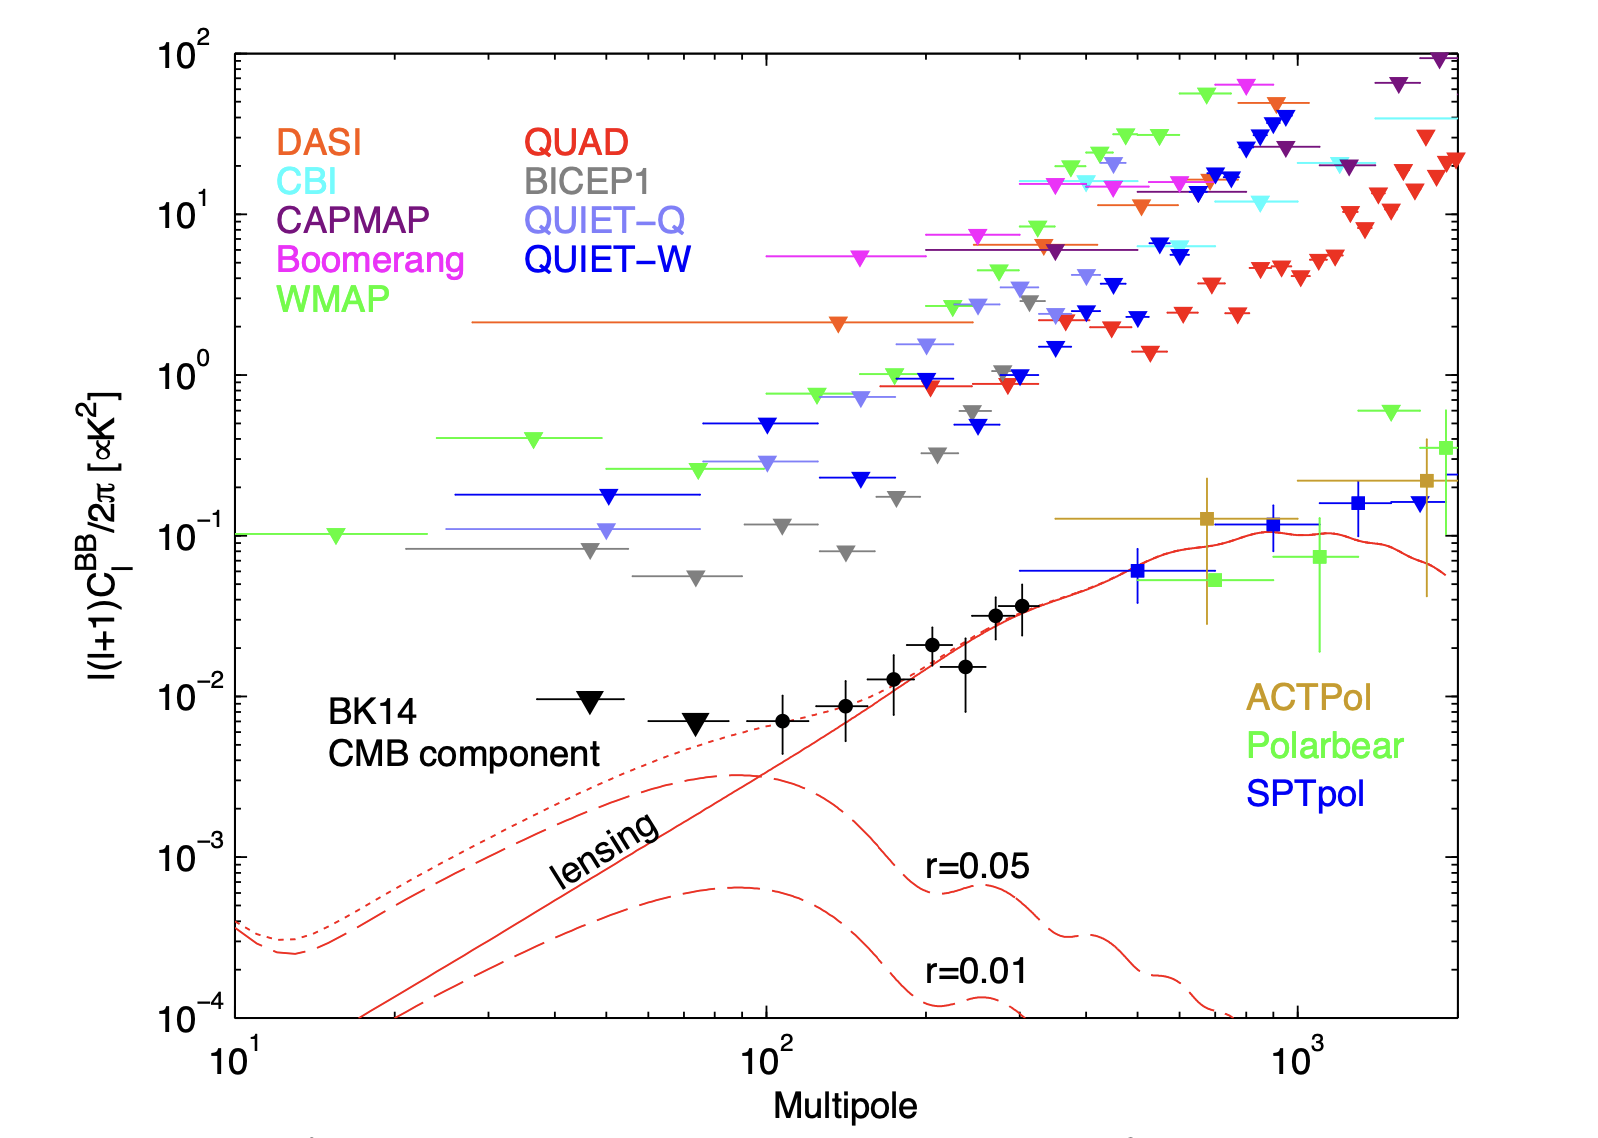
\includegraphics[width=0.8\columnwidth]{2_cosmology/figs/bicep_ref.png}
  \caption{偏光Bモードパワースペクトルの理論予想\cite{bicep_Bmode}。重力レンズ由来のBモードスペクトルは原始重力波由来のものと振る舞いが異なる。また、テンソル$\cdot$スカラー比の値によってもスペクトルの大きさが異なる。}
  \label{bicep_paper}
\end{figure}
原始重力波由来のBモードと重力レンズ由来のBモードはスペクトルの$\ell$依存性の違いから区別できる。また、原始重力波由来のBモード探索は重力レンズの影響が少ない大角度スケールで行う必要がある。原始重力波の振幅は慣例的にスカラー型揺らぎの振幅との比で表す。この比の値を``テンソル$\cdot$スカラー比''$r$と呼ぶ。波数$q$に対して、原始重力波とスカラー型揺らぎのパワースペクトルをそれぞれ$P_{重力波}(q)$、$P_{スカラー}(q)$とすると$r$は
\begin{equation}
  r(q) = \frac{4P_{重力波}(q)}{P_{スカラー}(q)}
\end{equation}
と表せる。インフレーションの発見は偏光Bモードのパワースペクトルを得ること、すなわち0ではないテンソル$\cdot$スカラー比の発見であり、多くのCMB実験によってこの$r$に対する制限が与えられている。現在ではPlanck衛星の結果にBICEP/Keck実験の観測結果を加えたもので、$r$に対して
\begin{equation}
  r(q=\SI{0.05}{\mathrm{Mpc}^{-1}}) < 0.036 ~ (\SI{95}{\%} ~\mathrm{Confidence~Level})
\end{equation}
という上限が与えられている\cite{const_r}。
\begin{figure}[htbp]
  \centering
  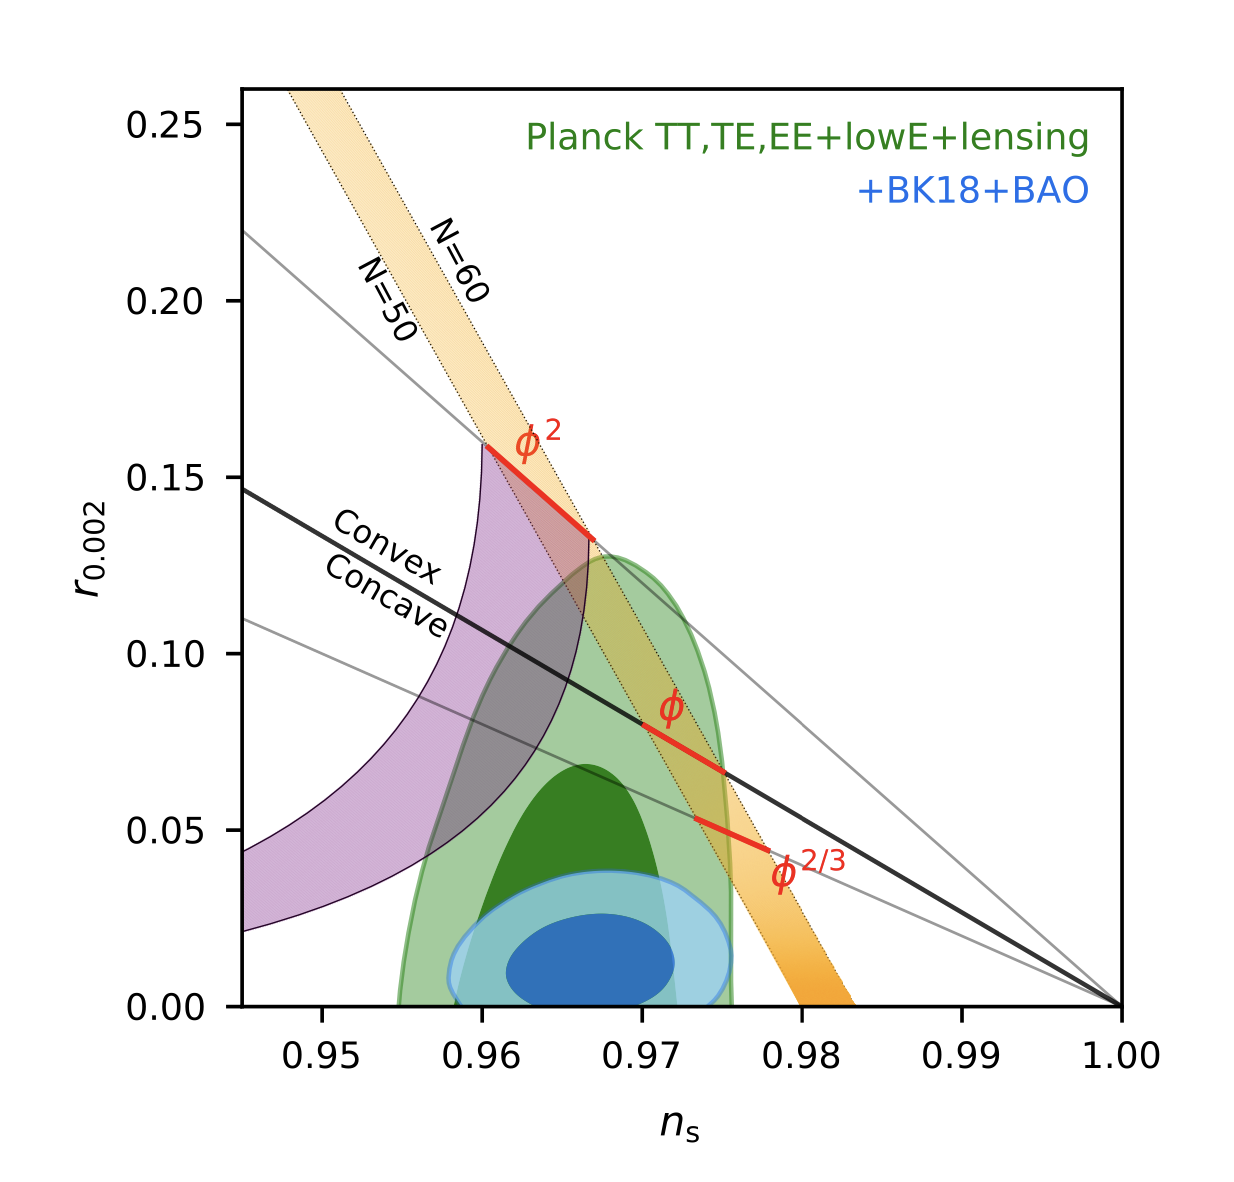
\includegraphics[width=0.6\columnwidth]{2_cosmology/figs/latest_results.png}
  \caption{Planck実験とBICEP/Keck実験によって与えられた$r$と$n_{s}$平面に付けられた制限\cite{const_r}。$n_{s}$はスカラー揺らぎを特徴付ける量で、この値が1からずれていることがインフレーションを支持することを意味する。$N$はインフレーションによるスケールファクターの膨張率を表す。また、実線でインフラトンのポテンシャルが$\phi$の冪乗だと仮定した時の$r$と$n_{s}$の関係を示している。}
  \label{const_r}
\end{figure}

\section{CMBの偏光とニュートリノ質量和}

\subsection{宇宙の再電離と光学的厚み~$\tau$}
\label{reion_and_tau}
宇宙の晴れ上がり以降CMB光子は一切散乱されることはないかといえばそうではない。晴れ上がりの後、赤方偏移$z\sim 20$\footnote{赤方偏移$z$はスケールファクターに対して$1+z = \frac{1}{a}$の関係である。}の時期になると、最初の天体が誕生し、天体から発せられる強い紫外線によって宇宙に広がっていた中性水素原子が再び電離される。この現象を``宇宙の再電離''と呼ぶ。再電離によって生じた自由電子によってCMB光子は再び散乱される。この再電離期を特徴付けるパラメータとして光学的厚み$\tau$を
\begin{equation}
  \tau\equiv\int_{t_{rs}}^{t_{0}}dt\bar{n}_{e}\sigma_{\tau}
\end{equation}
と定義する。ここで、$t_{rs}$は再電離が開始した時間、$t_{0}$は現在の時刻、$\bar{n}_{e}$は自由電子の平均個数密度、$\sigma_{\tau}$はCMBと自由電子の散乱断面積を表す。つまり、光学的厚みはCMBにとって電子がどれほど不透明であったかを示す量である。

再電離期の散乱はCMBの異方性に角度スケールに応じて2つの効果をもたらす。1つは$\ell\gtrsim 10$の角度スケールでCMBの異方性が散乱によってならされて、パワースペクトルが$e^{-2\tau}$で減衰する効果である。もう1つは$\ell\lesssim 10$の大角度スケールで新しい偏光を作る効果で、偏光の強度は$1-e^{-\tau}\sim\tau$に比例する。パワースペクトルにすると、$\tau^{2}$に比例する。赤方偏移$z$で電子が見る四重極に寄与する波数が赤方偏移$z$でのハッブル長に対応する波数となる。$z$のハッブル長程度の波長より短波長の異方性はならされ、ハッブル長程度の波長で偏光が生じる。そのため、2つの効果の$\ell$依存性は再電離期のハッブル長に対応している。また、$\ell\lesssim 10$での効果は偏光Eモードのパワースペクトルに対して現れる。

\subsection{ニュートリノ質量和との縮退}
光学的厚み$\tau$は宇宙の再電離期を特徴付ける他にもニュートリノ質量和($\Sigma m_{\nu}$)を知る手掛かりにもなる。光学的厚み$\tau$とニュートリノ質量和($\Sigma m_{\nu}$)はともにその値によって$\ell\sim 1000$の小角度スケールで観測される重力レンズ由来のBモードパワースペクトルの振幅を変える(図\ref{tau_mass})。
\begin{figure}[htbp]
  \centering
  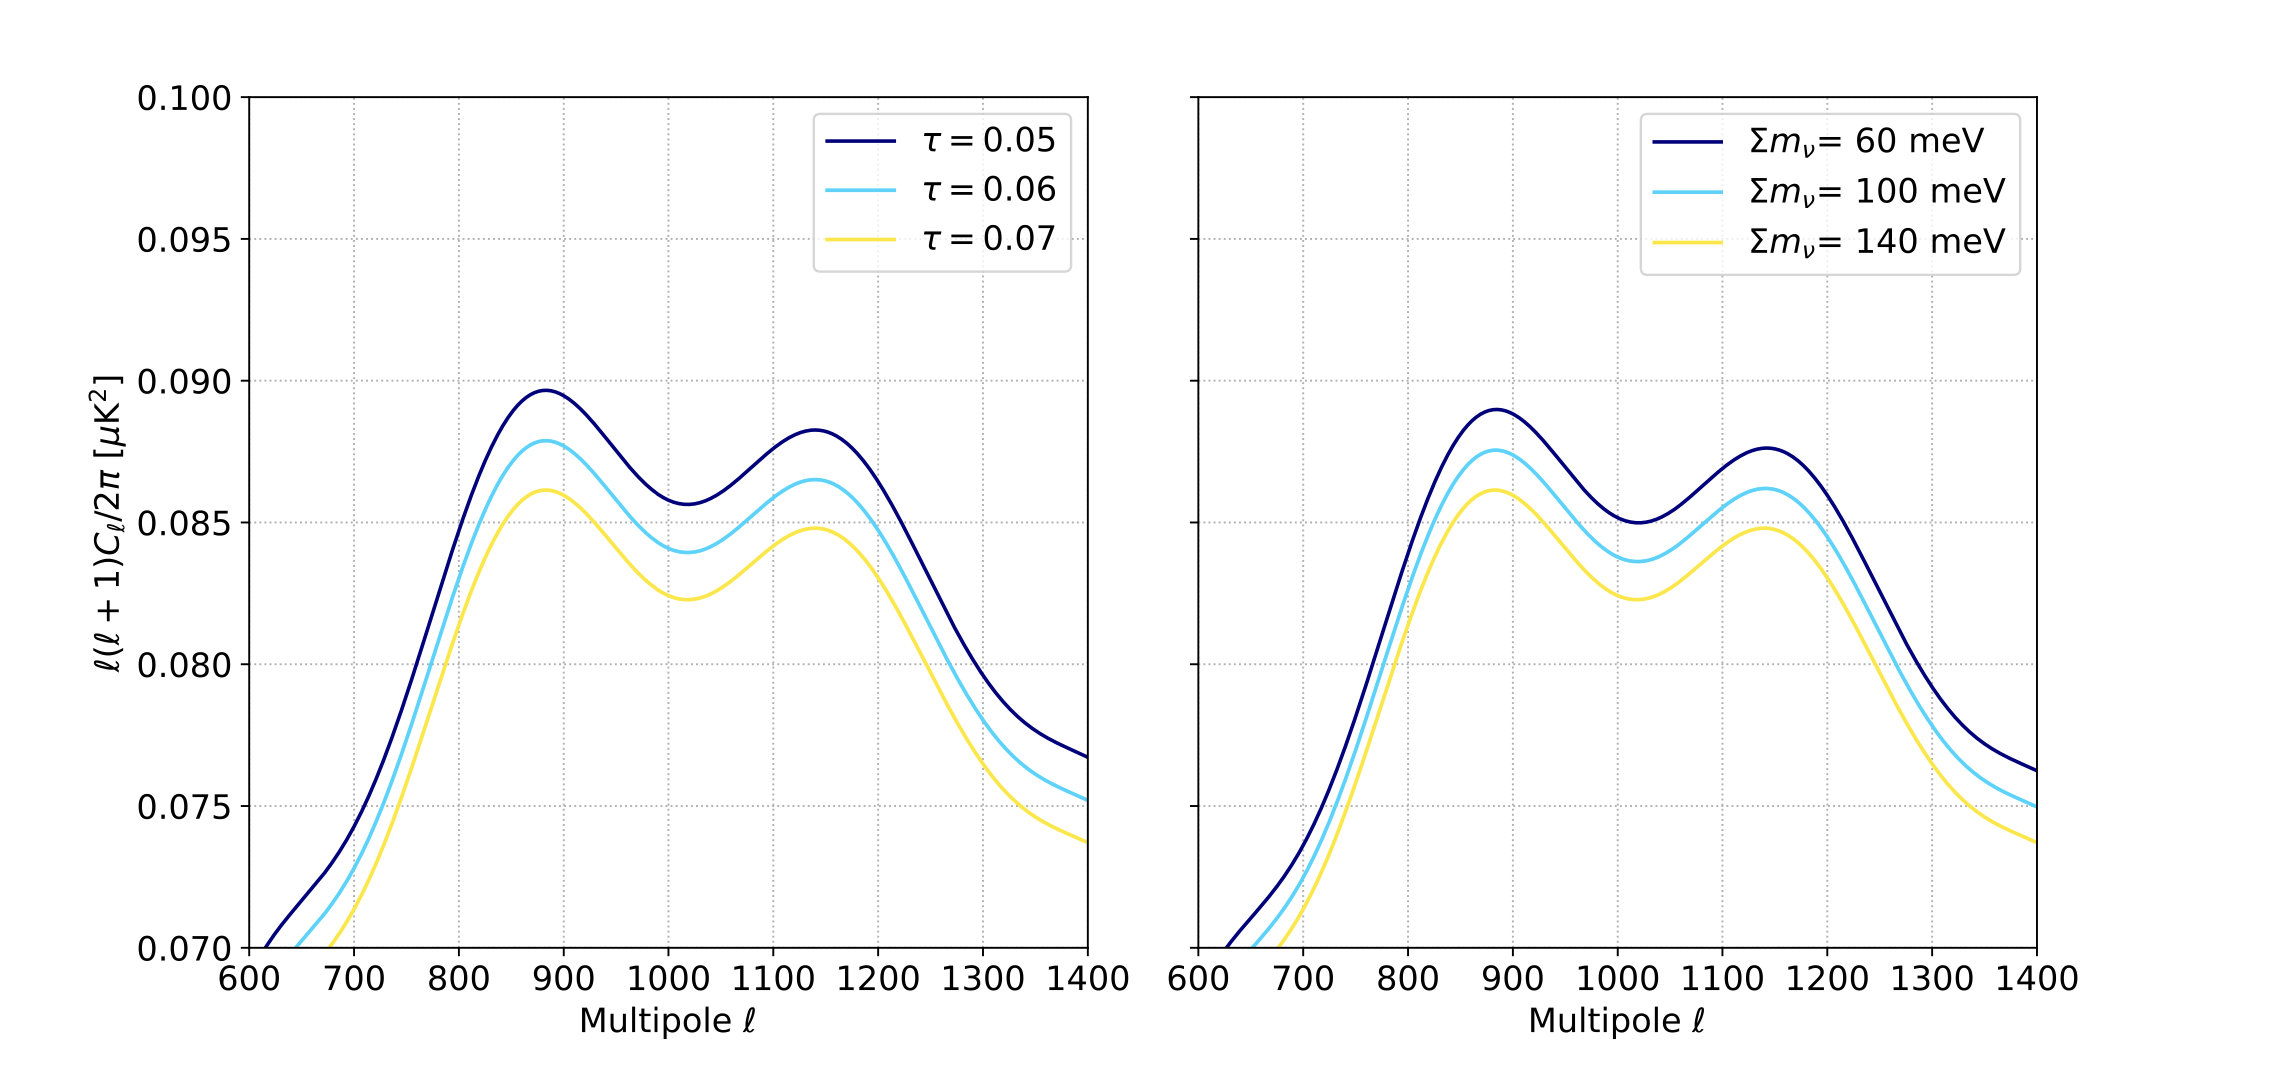
\includegraphics[width=1.0\columnwidth]{2_cosmology/figs/tau_mass.png}
  \caption{$\tau$、$\Sigma m_{\nu}$によって変化する重力レンズBモードパワースペクトル。\cite{sueno_doctor}より引用。}
  \label{tau_mass}
\end{figure}
$\tau$の値が大きいほど、また$\Sigma m_{\nu}$が大きいほどスペクトルの振幅は小さくなる。ニュートリノは速度分散が大きく、小角度スケールでは構造形成を抑制するように働く。そのため、重力レンズによる影響も抑制される。この効果が質量和に応じて異なるため、スペクトルの振幅に違いが生まれる。$\tau$に関しても、同様な効果を生むため両者は縮退したパラメータとなっている。そのため、$\tau$を精度良く測定することで$\Sigma m_{\nu}$との縮退を解くことができる(図\ref{degeneracy})。ニュートリノの質量和は素粒子物理学においても重要な課題であり、CMBの偏光観測からこの課題に迫れることは大きな意義がある。
\begin{figure}[htbp]
  \centering
  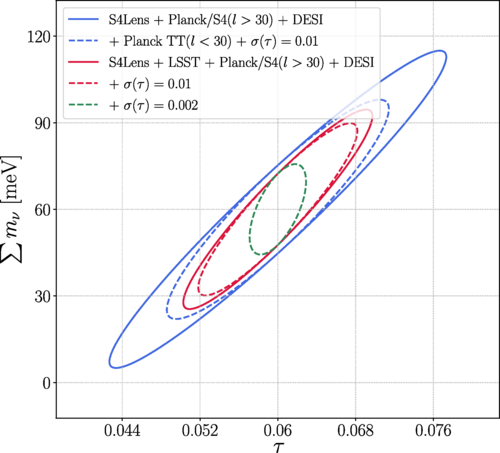
\includegraphics[width=0.75\columnwidth]{2_cosmology/figs/medium.png}
  \caption{縮退した$\tau$と$\Sigma m_{\nu}$。図の楕円は$1\sigma$のConfidence Levelを表す。\cite{degeneracy}より引用。}
  \label{degeneracy}
\end{figure}

\subsection{偏光Eモードと$\tau$}
\label{E_and_tau}
\ref{reion_and_tau}節でも述べたように、重力レンズ由来のBモード以外にもEモードのパワースペクトルから$\tau$の値を測定することができる。再電離によって$\ell\lesssim 10$の大角度スケールでEモードのパワースペクトルに$\tau^{2}$の依存性を生む。つまり、$\tau$が大きいほどスペクトルの振幅が大きくなる。そのため、Eモードの観測から$\tau$を精度良く測定することでも$\Sigma m_{\nu}$との縮退を解くことができる。
温度異方性のパワースペクトルも含めてニュートリノ質量和に迫る$\tau$の測定方法をまとめると表\ref{tau_methods}のようになる。
\begin{table}[htbp]
  \centering
  \caption{$\tau$の測定が可能なパワースペクトルのモードと角度スケール。}
  \vspace{3mm}
  \begin{tabular}{cc} \hline
    モード & 角度スケール  \\ \hline
    温度異方性 & 小角度($\tau$がスカラー型の原始揺らぎの振幅$A_{s}$と縮退するため単独では難しい) \\
    E & 大角度($\ell\lesssim 10$) \\
    B(重力レンズ) & 小角度($\ell\sim 1000$) \\ \hline
  \end{tabular}
  \label{tau_methods}
\end{table}
これより、偏光モードと角度スケールに応じて$\tau$、そして$\Sigma m_{\nu}$にアプローチすることができる。

\section{本論文の構成}
本論文の構成を述べる。第\ref{chapter1}章ではCMBに関わる理論的な背景を述べた。第\ref{chapter2}章でGroundBIRD実験の概要を説明する。以降は第\ref{chapter3}章と第\ref{chapter4_1}章から第\ref{chapter4_3}章までの2部構成になっており、第\ref{chapter3}章でGroundBIRDの角度データ取得システムの改善について述べる。第\ref{chapter4_1}章で焦点面検出器のアライメントの課題の定量化とその較正方針について述べる。第\ref{chapter4_2}章で課題に対する実際の取り組みと天体を用いた較正結果を述べ、第\ref{chapter4_3}章で差分解析によって確認した大気揺らぎの抑制について述べる。第\ref{chapter5}章で今後の展望を述べ、第\ref{chapter6}章でまとめを述べる。
